\documentclass[10pt]{exam}
\usepackage[phy]{template-for-exam}
\usepackage{pgfplots}
\pgfplotsset{
    compat=1.18,
    reg/.append style={
        xmin =-4.5,
        xmax =4.5,
        ymin =-4.5,
        ymax = 4.5,
        axis lines = center,
        xtick = {-4,...,4},
        ytick = {-4,...,4},
        height = 6cm,
        width = 6cm,
        grid = major,
        grid style = {thick, dotted},
        tick label style = {font=\small}
      },
    pulseplot/.append style={
      xmin =-6.5,
      xmax = 6.5,
      ymin =-2.5,
      ymax = 2.5,
      axis lines = center,
      xtick = {-6,...,6},
      ytick = {-2,...,2},
      height = 5cm,
      width = 7.5cm,
      grid = major,
      grid style = {thick, dotted},
      tick label style = {font=\small}
    },
    myplot/.append style={
      smooth,domain=-6:6,samples=50,thick
    },
  }
\pgfmathdeclarefunction{gauss}{2}{%
  \pgfmathparse{1/(#2*sqrt(2*pi))*exp(-((x-#1)^2)/(2*#2^2))}%
}

\title{Reading Guide - Interference}
\author{Rohrbach}
\date{\today}

\begin{document}
\maketitle

\begin{questions}


\question
  What is interference?
  \vs

\question
  What are the two types of interference?
  \vs

\question
  Draw each of the forms of interference below:

  \vspace{2em}


  \begin{tikzpicture}
    \def\plotsep{4}

    \draw (6.5,3)  -- ++(0,-15);

    \begin{scope}
      \begin{scope}
        \node[anchor=east] at (0,1.8) {$t=\SI{0}{\second}$};
        \begin{axis}[pulseplot]
          \addplot[myplot, ultra thick] {1.3*(gauss(-4,.5)+gauss(4,.5))};
        \end{axis}
      \end{scope}
      
      \begin{scope}[shift={(0,-\plotsep)}]
        \node[anchor=east] at (0,1.8) {$t=\SI{1}{\second}$};
        \begin{axis}[pulseplot]
          \addplot[myplot, ultra thick] {1.3*(gauss(-2,.5)+gauss(2,.5))};
        \end{axis}
      \end{scope}
  
      \begin{scope}[shift={(0,-2*\plotsep)}]
        \node[anchor=east] at (0,1.8) {$t=\SI{2}{\second}$};
        \begin{axis}[pulseplot]
        \end{axis}
      \end{scope}


      \begin{scope}[shift={(0,-3*\plotsep)}]
        \node[anchor=east] at (0,1.8) {$t=\SI{3}{\second}$};
        \begin{axis}[pulseplot]
        \end{axis}
      \end{scope}
  
    \end{scope}

    \begin{scope}[shift={(8,0)}]
      \begin{scope}
        \node[anchor=east] at (0,1.8) {$t=\SI{0}{\second}$};
        \begin{axis}[pulseplot]
          \addplot[myplot, ultra thick] {1.3*(gauss(-4,.5)-gauss(4,.5))};
        \end{axis}
      \end{scope}
      
      \begin{scope}[shift={(0,-\plotsep)}]
        \node[anchor=east] at (0,1.8) {$t=\SI{1}{\second}$};
        \begin{axis}[pulseplot]
          \addplot[myplot, ultra thick] {1.3*(gauss(-2,.5)-gauss(2,.5))};
        \end{axis}
      \end{scope}
  
      \begin{scope}[shift={(0,-2*\plotsep)}]
        \node[anchor=east] at (0,1.8) {$t=\SI{2}{\second}$};
        \begin{axis}[pulseplot]
        \end{axis}
      \end{scope}


      \begin{scope}[shift={(0,-3*\plotsep)}]
        \node[anchor=east] at (0,1.8) {$t=\SI{3}{\second}$};
        \begin{axis}[pulseplot]
        \end{axis}
      \end{scope}
  
    \end{scope}
  \end{tikzpicture}


\question
  Draw the resulting wave in each of the following cases:


\begin{EnvUplevel}
  \begin{center}
    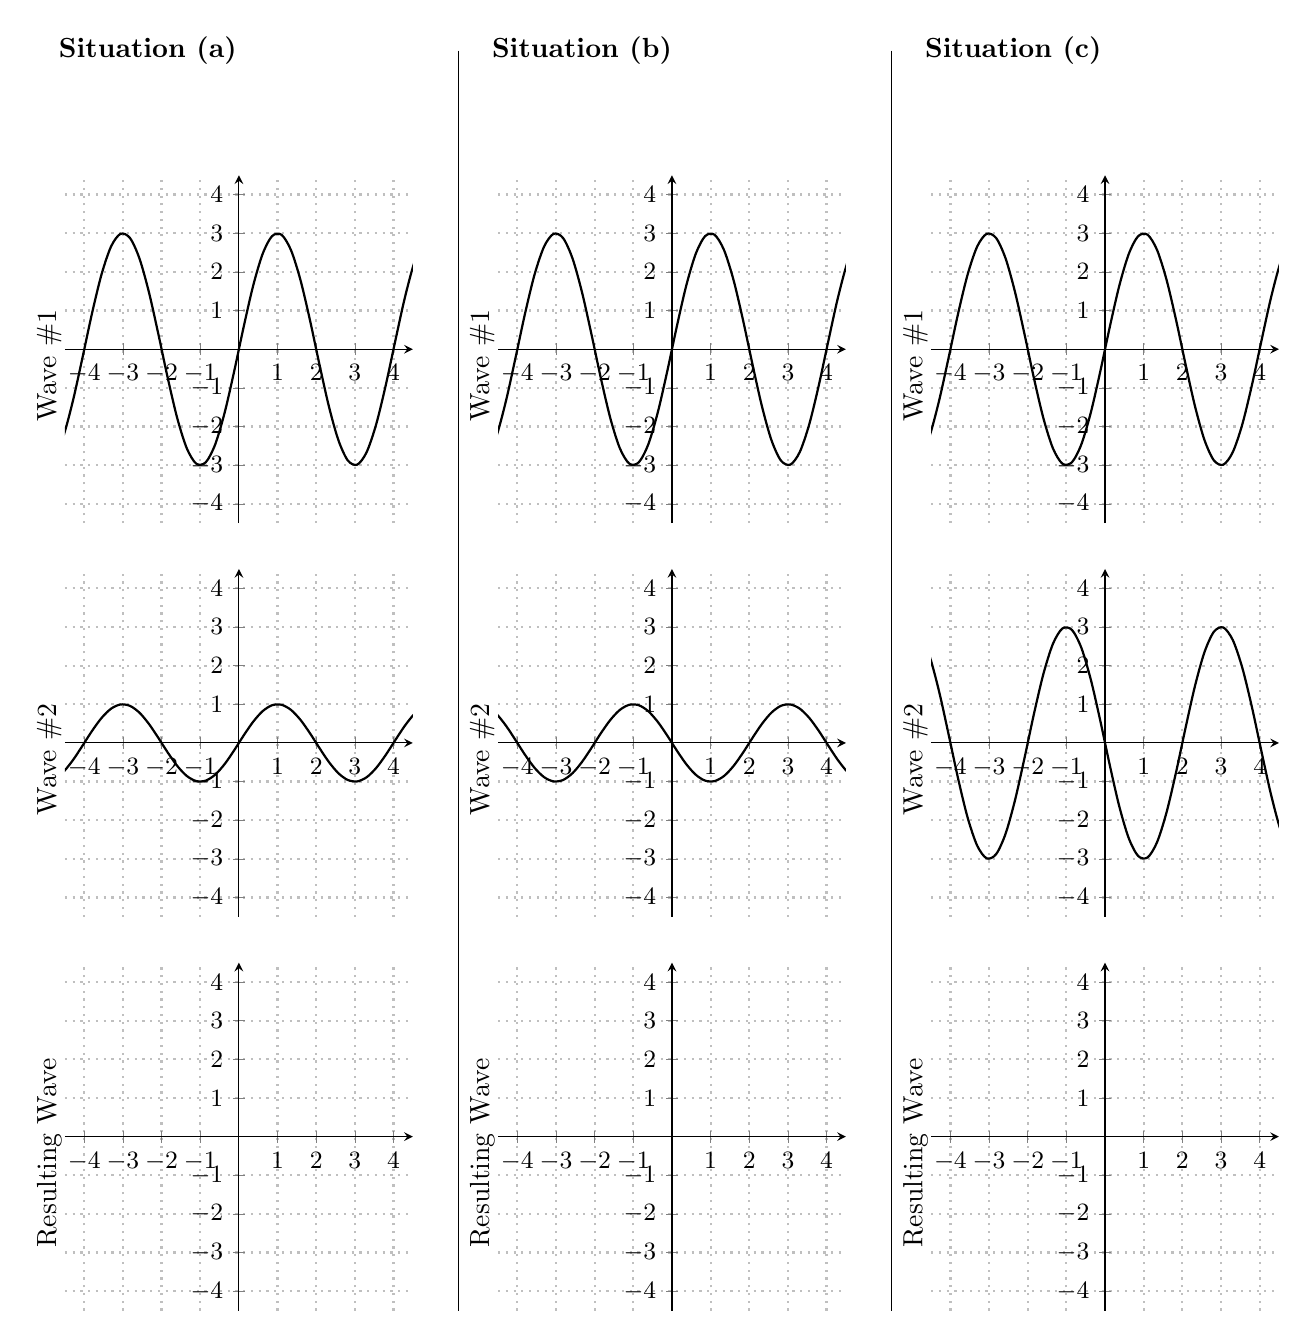
\begin{tikzpicture}
      \draw (5,6)  -- ++(0,-16);
      \draw (10.5,6)  -- ++(0,-16);
    
      \begin{scope}
        \node[anchor=west] at (-.2,6) {\bf Situation (a)};
        \begin{scope}
            \node[rotate=90] at (-.2,2) {Wave \#1};
            \begin{axis}[reg]
              \addplot[myplot] {3*sin(deg(2*pi*x/4))};
            \end{axis}
        \end{scope}
        
        \begin{scope}[shift={(0,-5)}]
          \node[rotate=90] at (-.2,2) {Wave \#2};
          \begin{axis}[reg]
            \addplot[myplot] {1*sin(deg(2*pi*x/4))};
          \end{axis}
        \end{scope}
    
        \begin{scope}[shift={(0,-10)}]
          \node[rotate=90] at (-.2,2) {Resulting Wave};
          \begin{axis}[reg]
          \end{axis}
        \end{scope}
    
      \end{scope}
        
      \begin{scope}[shift={(5.5,0)}]
    
        \node[anchor=west] at (-.2,6) {\bf Situation (b)};
        \begin{scope}
          \node[rotate=90] at (-.2,2) {Wave \#1};
            \begin{axis}[reg]
              \addplot[myplot] {3*sin(deg(2*pi*x/4))};
            \end{axis}
        \end{scope}
        
        \begin{scope}[shift={(0,-5)}]
          \node[rotate=90] at (-.2,2) {Wave \#2};
          \begin{axis}[reg]
            \addplot[myplot] {-1*sin(deg(2*pi*x/4))};
          \end{axis}
        \end{scope}
    
        \begin{scope}[shift={(0,-10)}]
          \node[rotate=90] at (-.2,2) {Resulting Wave};
          \begin{axis}[reg]
          \end{axis}
        \end{scope}
    
      \end{scope}
    
      \begin{scope}[shift={(11,0)}]
    
        \node[anchor=west] at (-.2,6) {\bf Situation (c)};
        \begin{scope}
          \node[rotate=90] at (-.2,2) {Wave \#1};
            \begin{axis}[reg]
              \addplot[myplot] {3*sin(deg(2*pi*x/4))};
            \end{axis}
        \end{scope}
        
        \begin{scope}[shift={(0,-5)}]
          \node[rotate=90] at (-.2,2) {Wave \#2};
          \begin{axis}[reg]
            \addplot[myplot] {-3*sin(deg(2*pi*x/4))};
          \end{axis}
        \end{scope}
    
        \begin{scope}[shift={(0,-10)}]
          \node[rotate=90] at (-.2,2) {Resulting Wave};
          \begin{axis}[reg]
          \end{axis}
        \end{scope}
    
      \end{scope}
    
    \end{tikzpicture}
  \end{center}
\end{EnvUplevel}

\end{questions}
\end{document}